\section{Really, what's SystemC?}
\mode<presentation>{
\begin{frame}
	\frametitle{Really, what's SystemC?}
	\begin{itemize}
		\item SystemC is proposed as a single ``\textbf{\textit{language}}'' to model your software/hardware platform at different layers of abstraction.
	\end{itemize}
	\begin{center}
		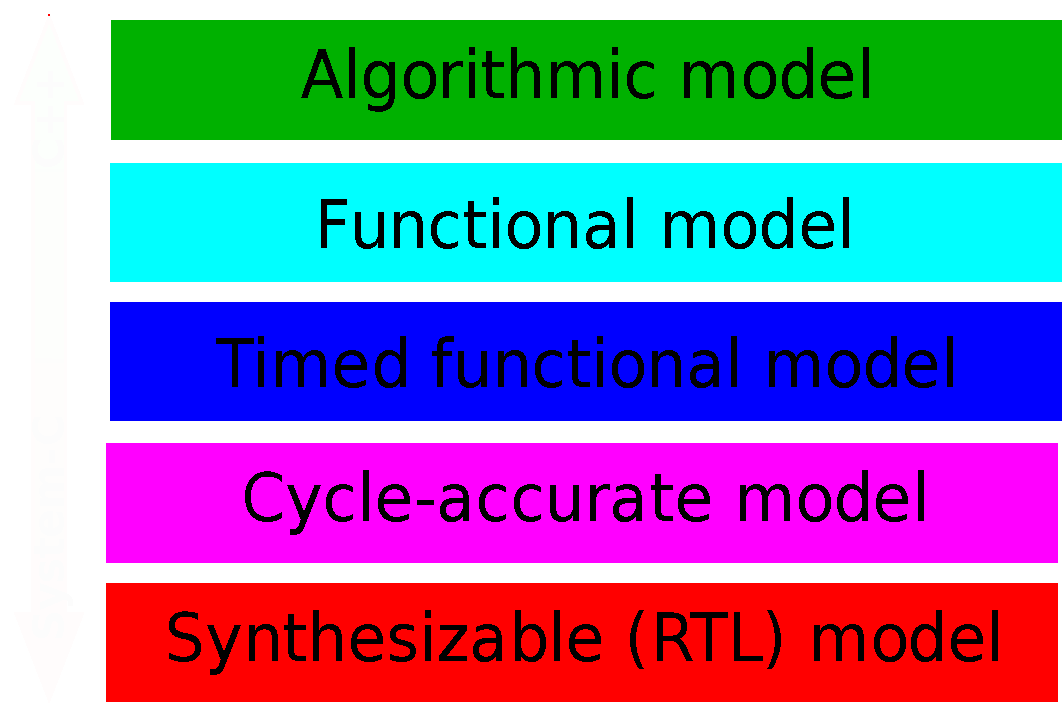
\includegraphics[width=0.8\textwidth]{introduction/figures/abstraction_layers-0.pdf}
	\end{center}
\end{frame}

\begin{frame}
\frametitle{Really, what's SystemC?}
	\begin{itemize}
		\item SystemC is proposed as a single ``\textbf{\textit{language}}'' to model your software/hardware platform at different layers of abstraction.
	\end{itemize}
	\begin{center}
		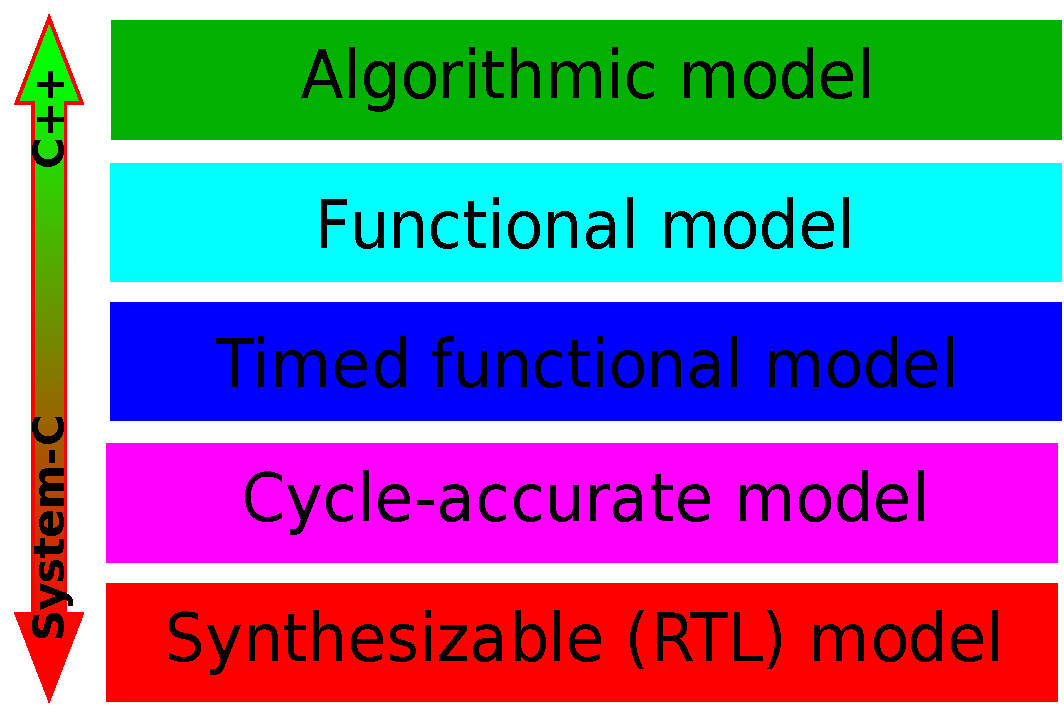
\includegraphics[width=0.8\textwidth]{introduction/figures/abstraction_layers-1.pdf}
	\end{center}
\end{frame}

\begin{frame}
	\frametitle{The abstraction levels: Algorithm}
	\begin{itemize}
		\item<1-> It defines what your system does.
		\item<1-> For example it can be described as a simple C++ program that computes Fibonacci.
	\end{itemize}
	\begin{figure}[h]
		\lstinputlisting{introduction/fibonacci.cc}
	\end{figure}
\end{frame}

\begin{frame}
	\frametitle{The abstraction levels: Functional}
	\begin{itemize}
		\item<1-> It defines how your system does what it is supposed to.
		\item<1-> The different system blocks appear at this stage.
		\item<1-> Continuing the Fibonacci example:
	\end{itemize}
	\begin{figure}[h]
		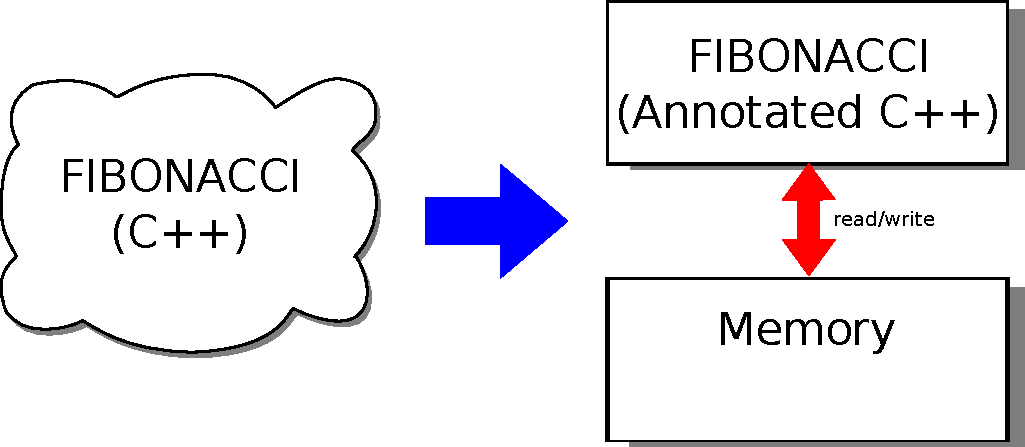
\includegraphics[width=0.8\textwidth]{introduction/figures/fibonacci_algo_to_functional_level.pdf}
	\end{figure}
\end{frame}

\begin{frame}
	\frametitle{The abstraction levels: Functional (II)}
	\begin{figure}[h]
		\lstinputlisting{introduction/fibonacci_annotated_presentation_1.cc}
	\end{figure}
\end{frame}

\begin{frame}
	\frametitle{The abstraction levels: Functional (II)}
	\begin{itemize}
		\item<1-> The {\color{red}read} and {\color{red}write} methods are responsible of sending messages using the SystemC primitives (which we will ignore for the moment).
	\end{itemize}
	\begin{figure}[h]
		\lstinputlisting{introduction/fibonacci_annotated_presentation_2.cc}
	\end{figure}
\end{frame}

\begin{frame}
	\frametitle{The abstraction levels: Timed functional}
	\begin{itemize}
		\item<1-> Adds time to the functional model, allowing you to model concurrency and resources constraints of your system. 
		\item<1-> The time description does not need to be precise,for example you can use average access times.
	\end{itemize}
	\begin{figure}[h]
		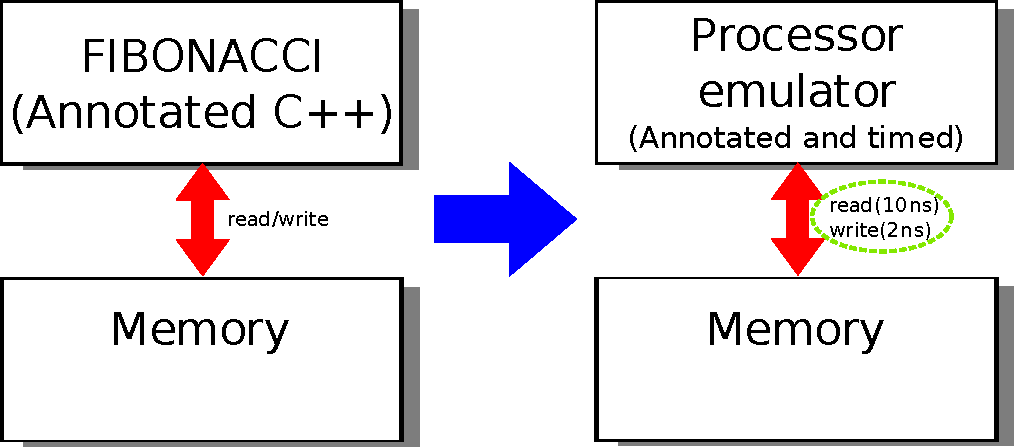
\includegraphics[width=0.8\textwidth]{introduction/figures/fibonacci_functional_to_timed_level.pdf}
	\end{figure}
\end{frame}

\begin{frame}
	\frametitle{The abstraction levels: Cycle-accurate}
	\begin{itemize}
		\item<1-> At this level time is very detailed, and matches closely that of the final system.
		\item<1-> Modeling at this level may require to write a new functional model.
	\end{itemize}
	\begin{figure}[h]
		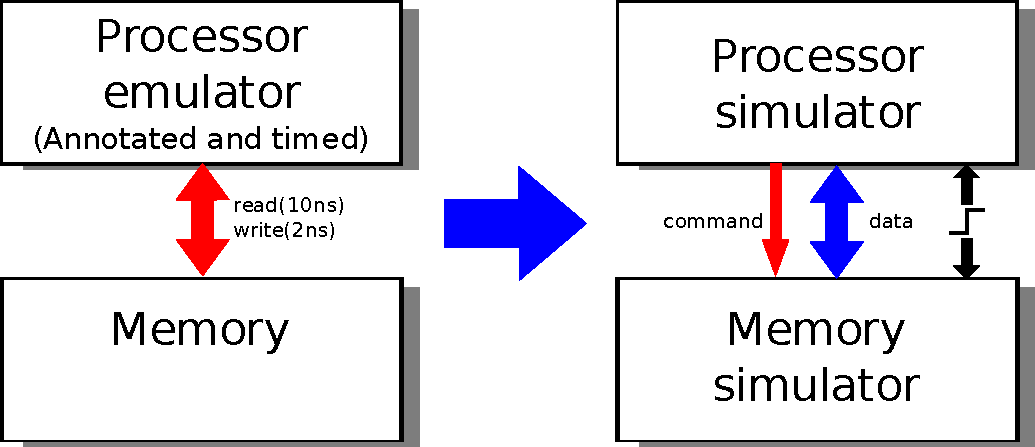
\includegraphics[width=0.8\textwidth]{introduction/figures/fibonacci_timed_to_cycle_level.pdf}
	\end{figure}
\end{frame}

\begin{frame}
	\frametitle{The abstraction levels: Synthesizable (RTL)}
	\begin{itemize}
		\item<1-> At this level the description is so detailed that the system can be synthetized.
	\end{itemize}
	\begin{figure}[h]
		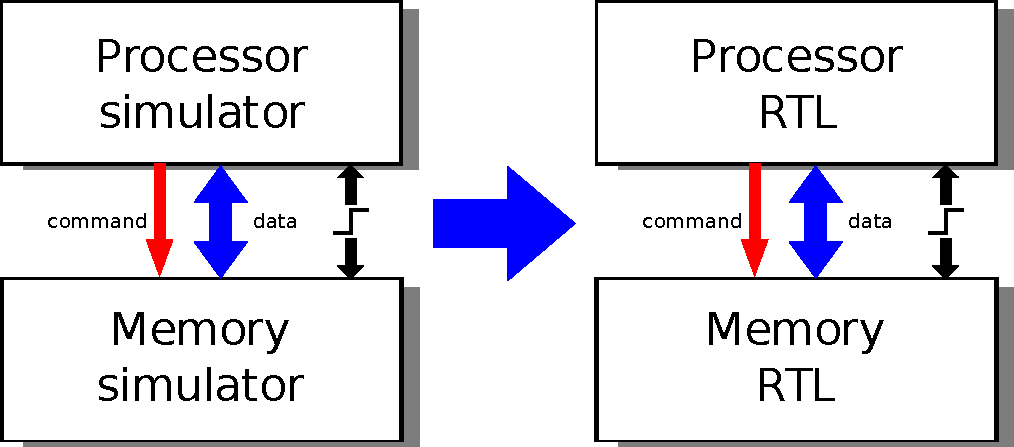
\includegraphics[width=0.8\textwidth]{introduction/figures/fibonacci_cycle_to_rtl_level.pdf}
	\end{figure}
\end{frame}
}

\mode<article>{
% \begin{figure}[!h]
% 	\begin{center}
% 		\includegraphics[page=6,height=6cm]{main_beamer.pdf}
% 	\end{center}
% 	\caption{Really, what's SystemC?}
% \end{figure}

\begin{figure}[!h]
	\begin{center}
		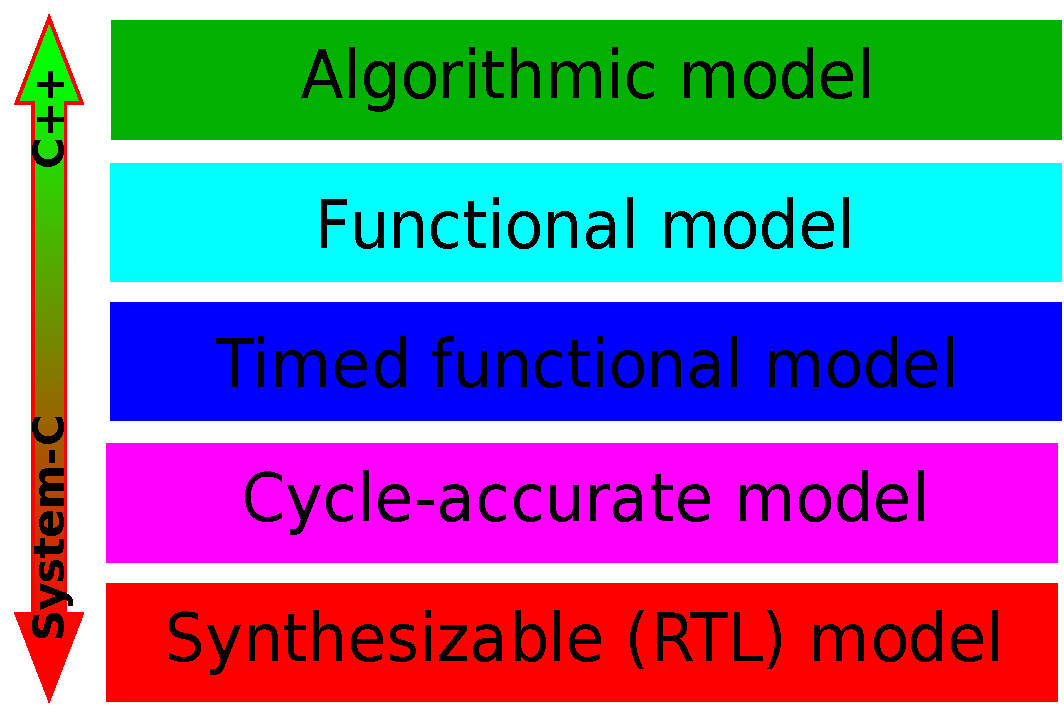
\includegraphics[width=0.8\textwidth]{introduction/figures/abstraction_layers-1.pdf}
	\end{center}
	\caption{Typical modeling levels of abstraction.}
	\label{fig:abstraction_layers}
\end{figure}

SystemC provides us with a single \emph{``language''} that allows us to model software/hardware platforms at different levels of abstraction.
Figure~\ref{fig:abstraction_layers} shows typical levels of abstraction when modeling software/hardware systems:
\begin{description}
	\item[Algorithm level:] it defines what your system does.
		For example, the algorithms implying the decoding of an MPEG4 flow into images.
	\item[Functional level:] it defines how your system does what it is supposed to do.
		Here you start to define the different blocks that compose your system: memories, processing elements, their connections, \ldots.
		Then you define how they communicate with each other, that is what is the communication sequence between your system components.
	\item[Timed functional level:] this model adds time to the functional model, allowing you to model concurrency and resources constraints of your system.
		The time description does not need to be precise, for example you can use average access times.
	\item[Cycle-accurate level:] this could be described as a very accurate timed functional model.
	\item[Synthetizable (RTL) level:] up to this level of abstraction, the description of components that composed the system did not need to be synthetizable.
		This level of abstraction provides a system that can be produced.
\end{description}

\begin{figure}[htb]
	\begin{center}
		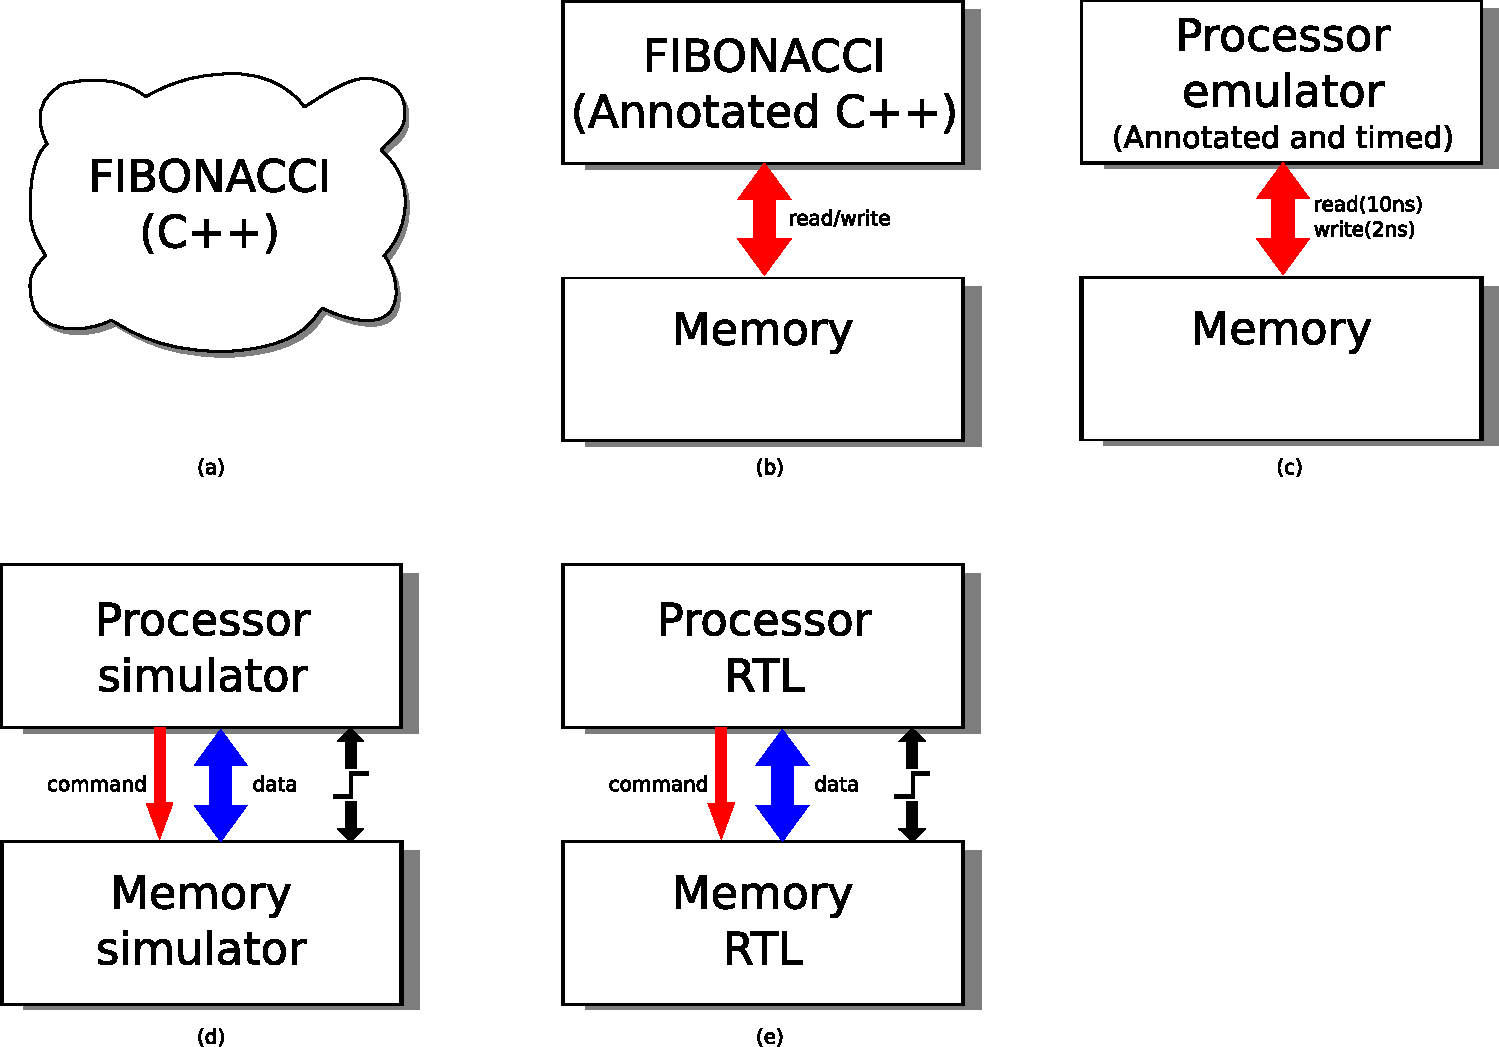
\includegraphics[width=0.8\textwidth]{introduction/figures/abstraction_level_example.pdf}
	\end{center}
	\caption{Example of a system represented at different levels of abstraction: (a) algorithm, (b) functional, (c) timed functional, (d) cycle-accurate, and (e) synthetizable levels.}
	\label{fig:abstraction_level_example}
\end{figure}

As SystemC is defined as an extension of the C++ programming language, the more abstract you are (the closer you are to the algorithm model) the less dependent you are in SystemC.
The more concrete your model is the more it will depend on SystemC. 
Actually, an algorithm model might be purely written in C++ without using any SystemC extensions.
Figure~\ref{fig:abstraction_level_example} shows an example of a system (that performs a simple Fibonacci) described using different levels of abstraction:
\begin{figure}[h]
	\lstinputlisting{introduction/fibonacci.cc}
	\caption{Fibonacci C/C++ program.}
	\label{fig:fibonacci_cpp_program}
\end{figure}
\begin{figure}[h]
	\lstinputlisting{introduction/fibonacci_annotated.cc}
	\caption{Annotated C/C++ program with SystemC calls.}
	\label{fig:annotated_fibonacci_cpp_program}
\end{figure}
\begin{itemize}
	\item (a) at \emph{algorithm} level of abstraction you start with a simple C++ program that performs Fibonacci, see Figure~\ref{fig:fibonacci_cpp_program}.
	\item (b) at \emph{functional} level you have decomposed your system into the different components that will compose your final system, and describe their communications.
		Note that the components do not need to be described precisely, they only need to provide functional descriptions.
		For example the processor component does not need to be a processor description, but it can be simply an annotated version of the Fibonacci program (see Figure~\ref{fig:annotated_fibonacci_cpp_program}) describing which are the communications required with the memory component of your system.
		SystemC enhances C++ by providing some basic classes that you can use to describe your system at functional level, like: a module class, an interface class, thread primitives, \ldots
	\item (c) at \emph{timed functional} level you include the time required to perform the different actions of your system.
		For example you define that a read communication between your processor and the memory takes 3ns, or that an addition takes only 0.01ns.
		At this step you may start to use slightly more detailed components, like processor emulators, which are able to execute real binaries.
		Thanks to these emulators you may know exactly how many additions are performed for your target processor architecture.
		Again, SystemC provides you classes to handle time in your system.
	\item (d) at \emph{cycle-accurate} level you start to define exactly what your system makes at each system clock signal.
		For example, at this point, you will use some kind of processor simulator, which is able to perform out-of-order and speculative execution, and capable of execute real binaries.
		Additionally, the communication protocol between the components needs to be exactly defined (no real hardware component understand something like: ``you have to perform a read''; instead you need to code your communication into buses, where the operation that you want to perform will be encoded, like for example in binary ``1'' could mean that the operation is a read, and ``0'' a write operation).
		Again, SystemC provides the classes you may need to describe your system.
	\item (e) at \emph{synthetizable} level your components will be replaced by SystemC descriptions that can be synthetizable.
		For example, up to this point your addition implementation had simply consisted on using the ``+'' C++ operator.
		You will have to replace it by the circuit description that performs the addition with the help of SystemC.
		\footnote{Synthetizable SystemC is still at its early stages. A working group is defining the SystemC language definitions that will allow you to do that. Additionally, libraries providing simple operators should start to appear (you do not want to define your ``+'' operation, usually you expect it to be provided by a library).}
\end{itemize}

Maybe those different levels seem very clear to you, however it is usually difficult to say when something starts being a functional model and stops being a simple algorithm, or a timed functional model a cycle-accurate one.
There is not a clear distinction between the levels, which makes difficult to define a model as belonging to a level or another.
So actually it will be up to you to decide if a model satifies your requirements or not based on the SystemC module description.

Models can mix components described at different levels. 
You can use a cycle-accurate component model and connect it to a functional component model, but usually you will need some kind of translators between the modules, that adds some kind of time to the communications from the functional model to the cycle-accurate one\footnote{Even if the time is just a ``fake''.}, and that abstracts the time from the cycle-accurate to the functional model.
However, you must bear in mind that if you mix two models with different abstraction levels, the final model will not be more accurate that the more abstract of your components.

}

\subsection{Scope of this document}

\mode<presentation>{
\begin{frame}
	\frametitle{Scope of this document}
	\begin{itemize}
		\item<1-> \emph{Coding styles} and not abstraction levels.
		\item<1-> This tutorial will focus on the following coding styles:
		\begin{itemize}
			\item<1-> Transaction Level Modeling (TLM):
			\begin{itemize}
				\item<1-> untimed
				\item<1-> loosely-timed
				\item<1-> approximately timed
			\end{itemize}
			\item<1-> Cycle Level Modeling (CLM)
		\end{itemize}
	\end{itemize}
%	\begin{figure}[h]
%		\includegraphics[width=0.8\textwidth]{introduction/figures/scope.pdf}
%	\end{figure}
\end{frame}
}

\mode<article>{
As we have seen SystemC can be used to model different levels of abstraction, however in this document we will focus on three of the previously presented levels of abstraction: functional, timed functional and cycle-accurate.
The SystemC community does not talk about abstraction levels, but instead they talk about coding styles. 
A single coding style could be used to implement a model in different abstraction levels, however it would be inefficient and tedious.
So at the end we can say that a coding style correspond to an abstraction level. 
The coding styles that correspond to the functional, timed functional and cycle-accurate abstraction levels are:
\begin{description}
	\item[Transaction Level Modeling (TLM):] SystemC groups under this name functional and timed functional levels. 
		The current specification is called TLM2.0 and it will soon follow a certification process (as SystemC itself which is an IEEE standard).
		SystemC proposes what are called three different coding styles:
		\begin{enumerate}
			\item untimed
			\item loosely-timed
			\item approximately timed
		\end{enumerate}
		We will study those coding styles and TLM2.0 more in detail later in this document.
	\item[Cycle Level Modeling (CLM):] Historically SystemC was created to model cycle level systems, and it is currently an IEEE standard.
		As you can imagine, this coding style is specially adapted to the cycle-accurate abstraction level.
\end{description}

As SystemC was initially developed with cycle level modeling in mind, and TLM was proposed later, in the following chapters we will start explaining CLM first.
However, before starting let's see a little bit how can you use SystemC in your projects and what does it include.

}

